\scanpage{50}
% archive sheet number: 49
% letterhead
U N I V E R S I T E\\
DES SCIENCES ET TECHNIQUES\\
DU LANGUEDOC\\
\texttt{-{}-{}-{}-{}-{}-{}-{}-{}-{}-{}-{}-}\\
Service de la Scolarité\\
MR/GJ\\
Diffusion : Liste H\\
N°3548

MONTPELLIER, le 8 JUIN 1978

% printed form
\uline{AVIS DE SOUTENANCE D'UNE THESE DE DOCTORAT D'ETAT}

\uline{Nom et prénom de la candidate} : LINDHEIMER née MONNIER Arlette

\uline{Titre de la thèse} : Contribution à l'étude diffusiomètrique des électrolytes dans des solvants mixtes de constantes diélectriques variables.

\uline{Date, heure et lieu de soutenance prévus} :\\
1er JUILLET 1978 à 9 Heures 30 mn\\
Salle de cours n° 2, U.S.T.L.

\uline{Nom du Directeur de thèse} : Monsieur le Professeur B. BRUN

\uline{Désignation du laboratoire où la thèse est préparée} :\\
Laboratoire des Interactions moléculaires, U.S.T.L.

\uline{Résumé de la thèse} : Les coefficients de diffusion ioniques ont été mesurés à 25°C pour des électrolytes dissous dans des solvants mixtes dont les constantes diélectriques prenaient des valeurs différentes :

- soit élevées comme dans les mélanges eau-N-méthylpropionamide,

- soit faibles comme dans les mélanges eau-alcool et eau-éther.

Dans le premier cas, la loi étendue relative au coefficient de diffusion a été vérifiée jusqu'à 0,2M environ ; dans les autres cas la présence d'associations ioniques a été mise en évidence et les paramètres d'associations ont été obtenus dans le cadre du modèle des paires d'ions.

\uline{Durée approximative des recherches ayant abouti à la thèse} : 5 ans

\uline{Noms des Rapporteurs} :

\diagram{\begin{tabular}{@{}l p{.70\linewidth}@{}}
SANFELD A. & Professeur, Chimie Physique, Univ. BRUXELLES\\
TURQ P. & Chargé de Cours, Chimie Physique, Univ. PARIS\\
BRUN B. & Professeur, Chimie Physique, U.S.T.L.
\end{tabular}}

\uline{Composition du jury} :

\diagram{\begin{tabular}{@{}l p{.70\linewidth}@{}}
BRUN B. & Professeur, Chimie Physique, Univ. Sciences et Techn. Languedoc MONTPELLIER\newline (Président)\\
SANFELD A. & Professeur, Chimie Physique, Univ. BRUXELLES\\
TURQ P. & Chargé de Cours, Chimie Physique, Univ. PARIS\newline (Membre extérieur choisi en raison de sa compétence scientifique)\\
GROMB S. & Professeur, Chimie Physique, U.S.T.L.\\
GIRAL L. & Professeur, Chimie Organique,U.S.T.L.\newline (Membre étranger à la spécialité de \unsure{:la|la} candidate)
\end{tabular}}

Le Secrétaire Général,\\
\handwritten{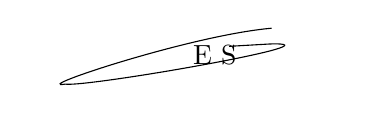
\begin{tikzpicture}[baseline=-.2ex,x=1cm,y=1cm]
\node at (1.95,.28) {\unsure{E S}};
\draw (.05,-.09) .. controls (-.42,-.16) and (1.64,.53) .. (2.67,.62);
\draw (.05,-.09) .. controls (.34,-.13) and (3.65,.45) .. (2.65,.42) -- (2.13,.39);
\end{tikzpicture}}\\
\uline{E. SIAU}

% printed form
MR LE PROFESSEUR GROTHENDIECK A.\\
MATHEMATIQUES\hspace{4cm}5

